%# -*- coding: utf-8-unix -*-
%%==================================================
%% chapter_2.tex for SJTU Master Thesis
%%==================================================

\chapter{IEEE1588协议原理分析研究}
\label{chap:1588_theory}
IEEE1588协议全名为:IEEE Standard for a Precision Clock Synchronization Portocol for Networked Measurement and Control Systems,也称为PTP精密时钟同步协议。PTP协议内部集成了多项分布式技术,如网络通信、局部计算和分布式对象等,对于所有支持多播局域网通信的分布式系统,尤其是以太网,都可以应用PTP协议来进行时钟同步。这可以在占用极少网络和本地计算资源的前提下,使得各类具有不同精确度、分辨率和稳定性的时钟同步且达到亚微秒级别的同步精度。

由于当今测控系统中越来越多的依赖分布式系统技术,而分布式系统的性能又极其依靠所有分布式节点之间的时钟同步精度。所以,一套优秀且能达到微秒甚至亚微秒级别的时钟同步协议显得尤为迫切,而IEEE1588协议的出现给这种需求带来了重要的影响,在相关领域也得到了非常快速的发展。

本章中会对IEEE1588时钟同步原理进行深入的分析研究,同时,也会对该协议中可能存在的一些严重问题进行分析,同时通过阅读文献来介绍关于这些问题的当今的一些研究理论成果,以期对IEEE1588协议原理及当前研究热点作一个较为立体而全面的分析。

\section{IEEE1588时钟同步过程}
一般而言,IEEE1588系统是由PTP设备和非PTP设备结合而成的分布式网络化系统。IEEE1588协议主要介绍的是系统中的实时PTP设备之间的相互同步方案,使得所有的从时钟能够与自己的主时钟同步,而所有主时钟又能够和同一个Grand Master时钟同步,最终达到整个系统中所有时钟保持同步。

首先,每个ptp时钟会有多个端口,当系统启动时,会立即开始主从秩序建立过程。该过程中,每个端口会对外发送Announce报文,同时通过检查所收到的Announce报文中的相关信息来判定哪个端口适合成为主时钟,被判定为主时钟的端口则会定期对外发送Sync报文。如果,一个判定为主时钟的端口收到了一个来自于更好的主时钟的Sync报文,那么该主时钟则会立即将自身的主时钟状态切换为从时钟状态。当然,如果一个处于从时钟状态的端口认为自己比当前主时钟更加好,那么它可以将自己设置为主时钟状态,并对外发送Sync报文。当所有端口通过互相比较时钟特性并建立了各自的主从状态后,则意味着主从秩序完成建立。如果此时新加入了一个时钟,那么该时钟首先会等待来自某一主时钟的Sync报文,若在规定的时间内没有收到任何主时钟的Sync报文,那么该时钟则将自身设置为主时钟,直到发现一个更好的主时钟。

随后,则会进行时钟同步过程。该过程主要是主从时钟之间发送报文,使得每个从时钟计算出自身与主时钟之间的时钟偏差,并且对自身进行校正从而实现同步。首先主时钟会对外界进行周期性的Sync报文发送,多数情况下该报文会将离开主时钟的时间戳标记进去。当从时钟收到Sync报文后,则能够接受到发送时间戳并记录当前的接收时间戳。但是,仅仅依靠这两个时间戳还不能够计算出真实的主从偏差,因为对于从时钟而言它并不知道自身与主时钟之间的链路传输延时。所以,从时钟自身也会周期性向主时钟发送Delay\_Request报文,会通过接受主时钟回传的Delay\_Resopnse报文来共同计算出链路延时delay和主从偏差offset。最终利用offset对从时钟进行校正而实现同步。

下面,详细介绍主从建立过程中及时钟同步过程中所应用到的算法,并对算法进行分析。

\subsection{最佳主时钟算法}
\label{sec:1588_theory_bmc}
由于ptp协议的核心是从时钟向主时钟同步从而最终实现整个系统时钟同步。所以,在真正的时钟同步之前,至关重要的一步便是建立全系统主从秩序,在该建立过程中,所有网络节点会通过“最佳主时钟算法(Best Master Clock Algorithm, BMC)”,选举出Grand Master Clock、主时钟、从时钟。其中,Grand Master Clock的精度最高,主时钟其次,从时钟最低。

下面进行简明扼要的最佳主时钟算法介绍。

当系统在启动之初,所有系统内部的时钟会对外发布Announce报文,该报文会包含自身时钟的与精度相关的特性。与此同时,所有时钟也会接受其他时钟发送过来的Announce报文,即接收到其他报文传递来的精度信息。

然后,每个端口内部会依据这些精度相关的数据集,在本地首先通过数据集比较算法,从而比较出两组数据的优劣,其中一组是时钟自身的缺省特性,另一组是来自外界其他时钟传递过来的数据。完成了数据集比较之后,会依靠比较结果继续执行状态决定算法。该算法会结合端口状态机规则及数据集比较结果来设置自身端口的主从状态。至此,每个时钟便已设置好了自身的主从状态,这其中最高级的主时钟便自动成为了Grand Master Clock。

具体拓扑结构可以参考下图:
\\
\\
\begin{figure}[htbp]
  \centering
  \begin{minipage}[b]{0.6\textwidth}
    \captionstyle{\centering}
    \centering
    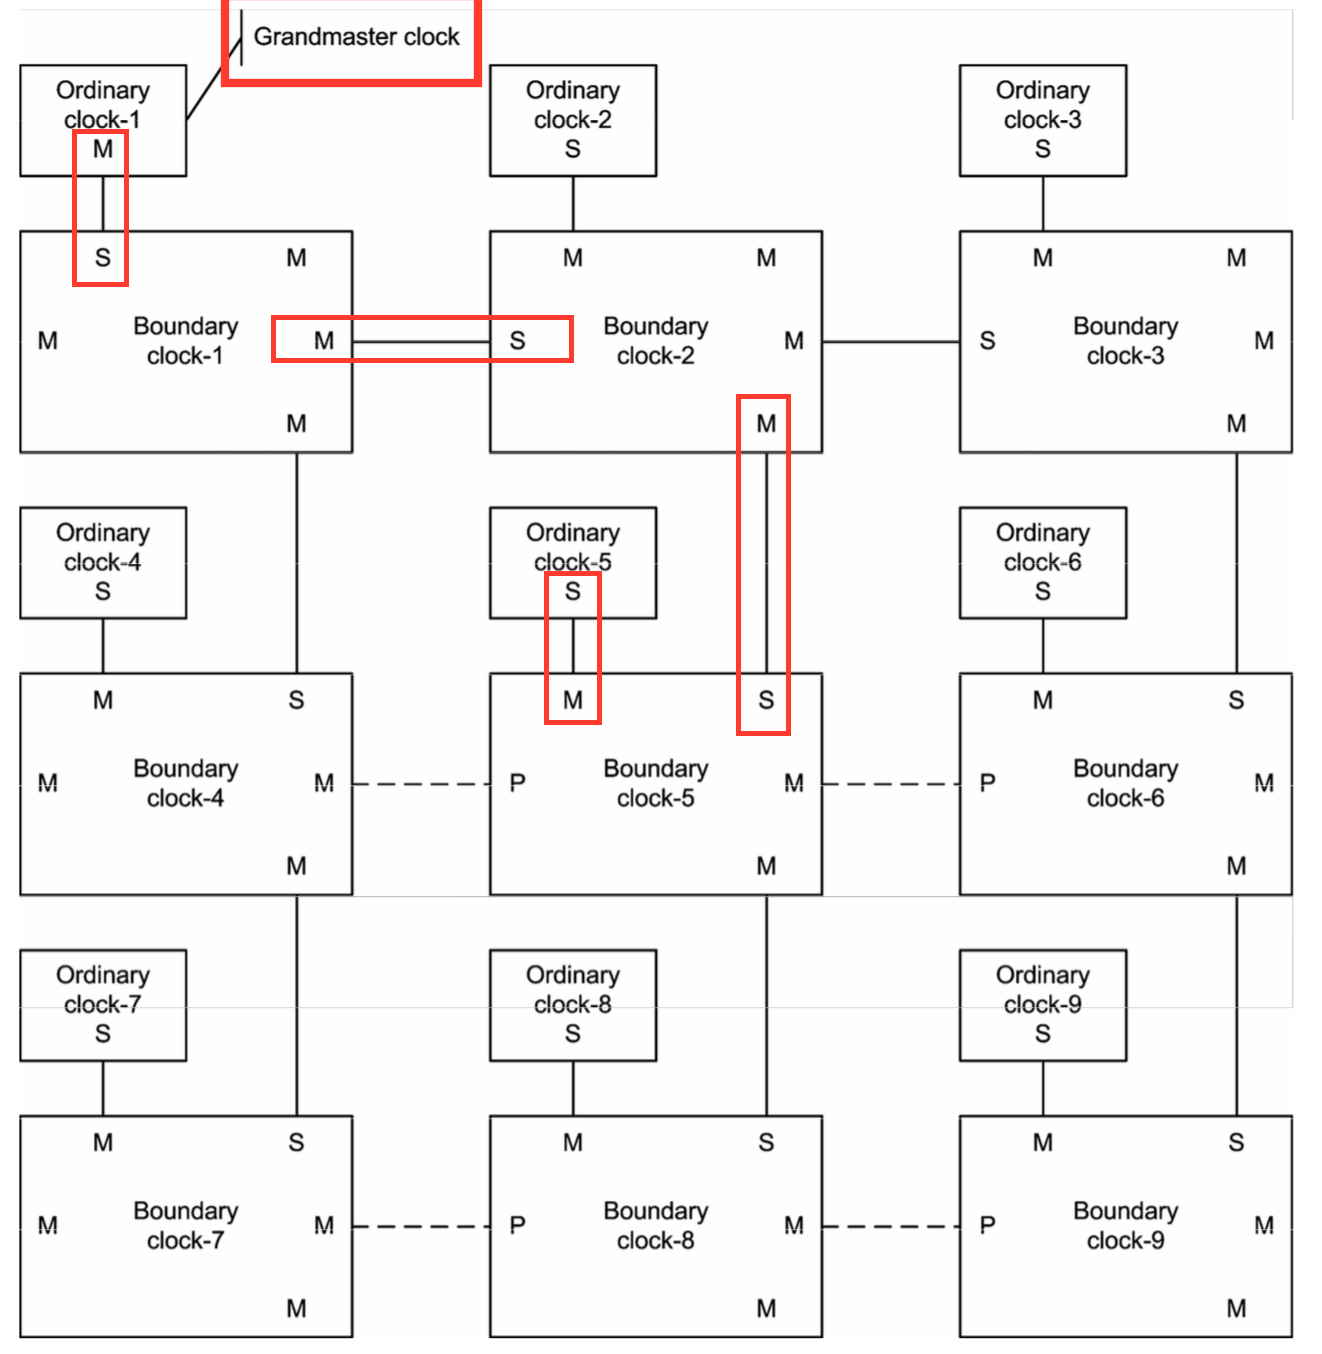
\includegraphics[width=10cm]{ptp_topo}
    \bicaption[fig:longcaptiongood]{PTP时钟同步拓扑结构}{PTP时钟同步拓扑结构}{Fig}{The topology of PTP Time-Sync System}
  \end{minipage}     
\end{figure}

\subsection{时钟同步算法}
\label{sec:1588_theory_sync}
在图\ref{fig:process_of_time_sync}中,可以看到较为完整的时钟同步过程。下面,对时钟同步过程及相关计算做简明扼要地介绍。

\begin{figure}[!hbp]
  \centering
  \begin{minipage}[b]{0.6\textwidth}
    \captionstyle{\centering}
    \centering
    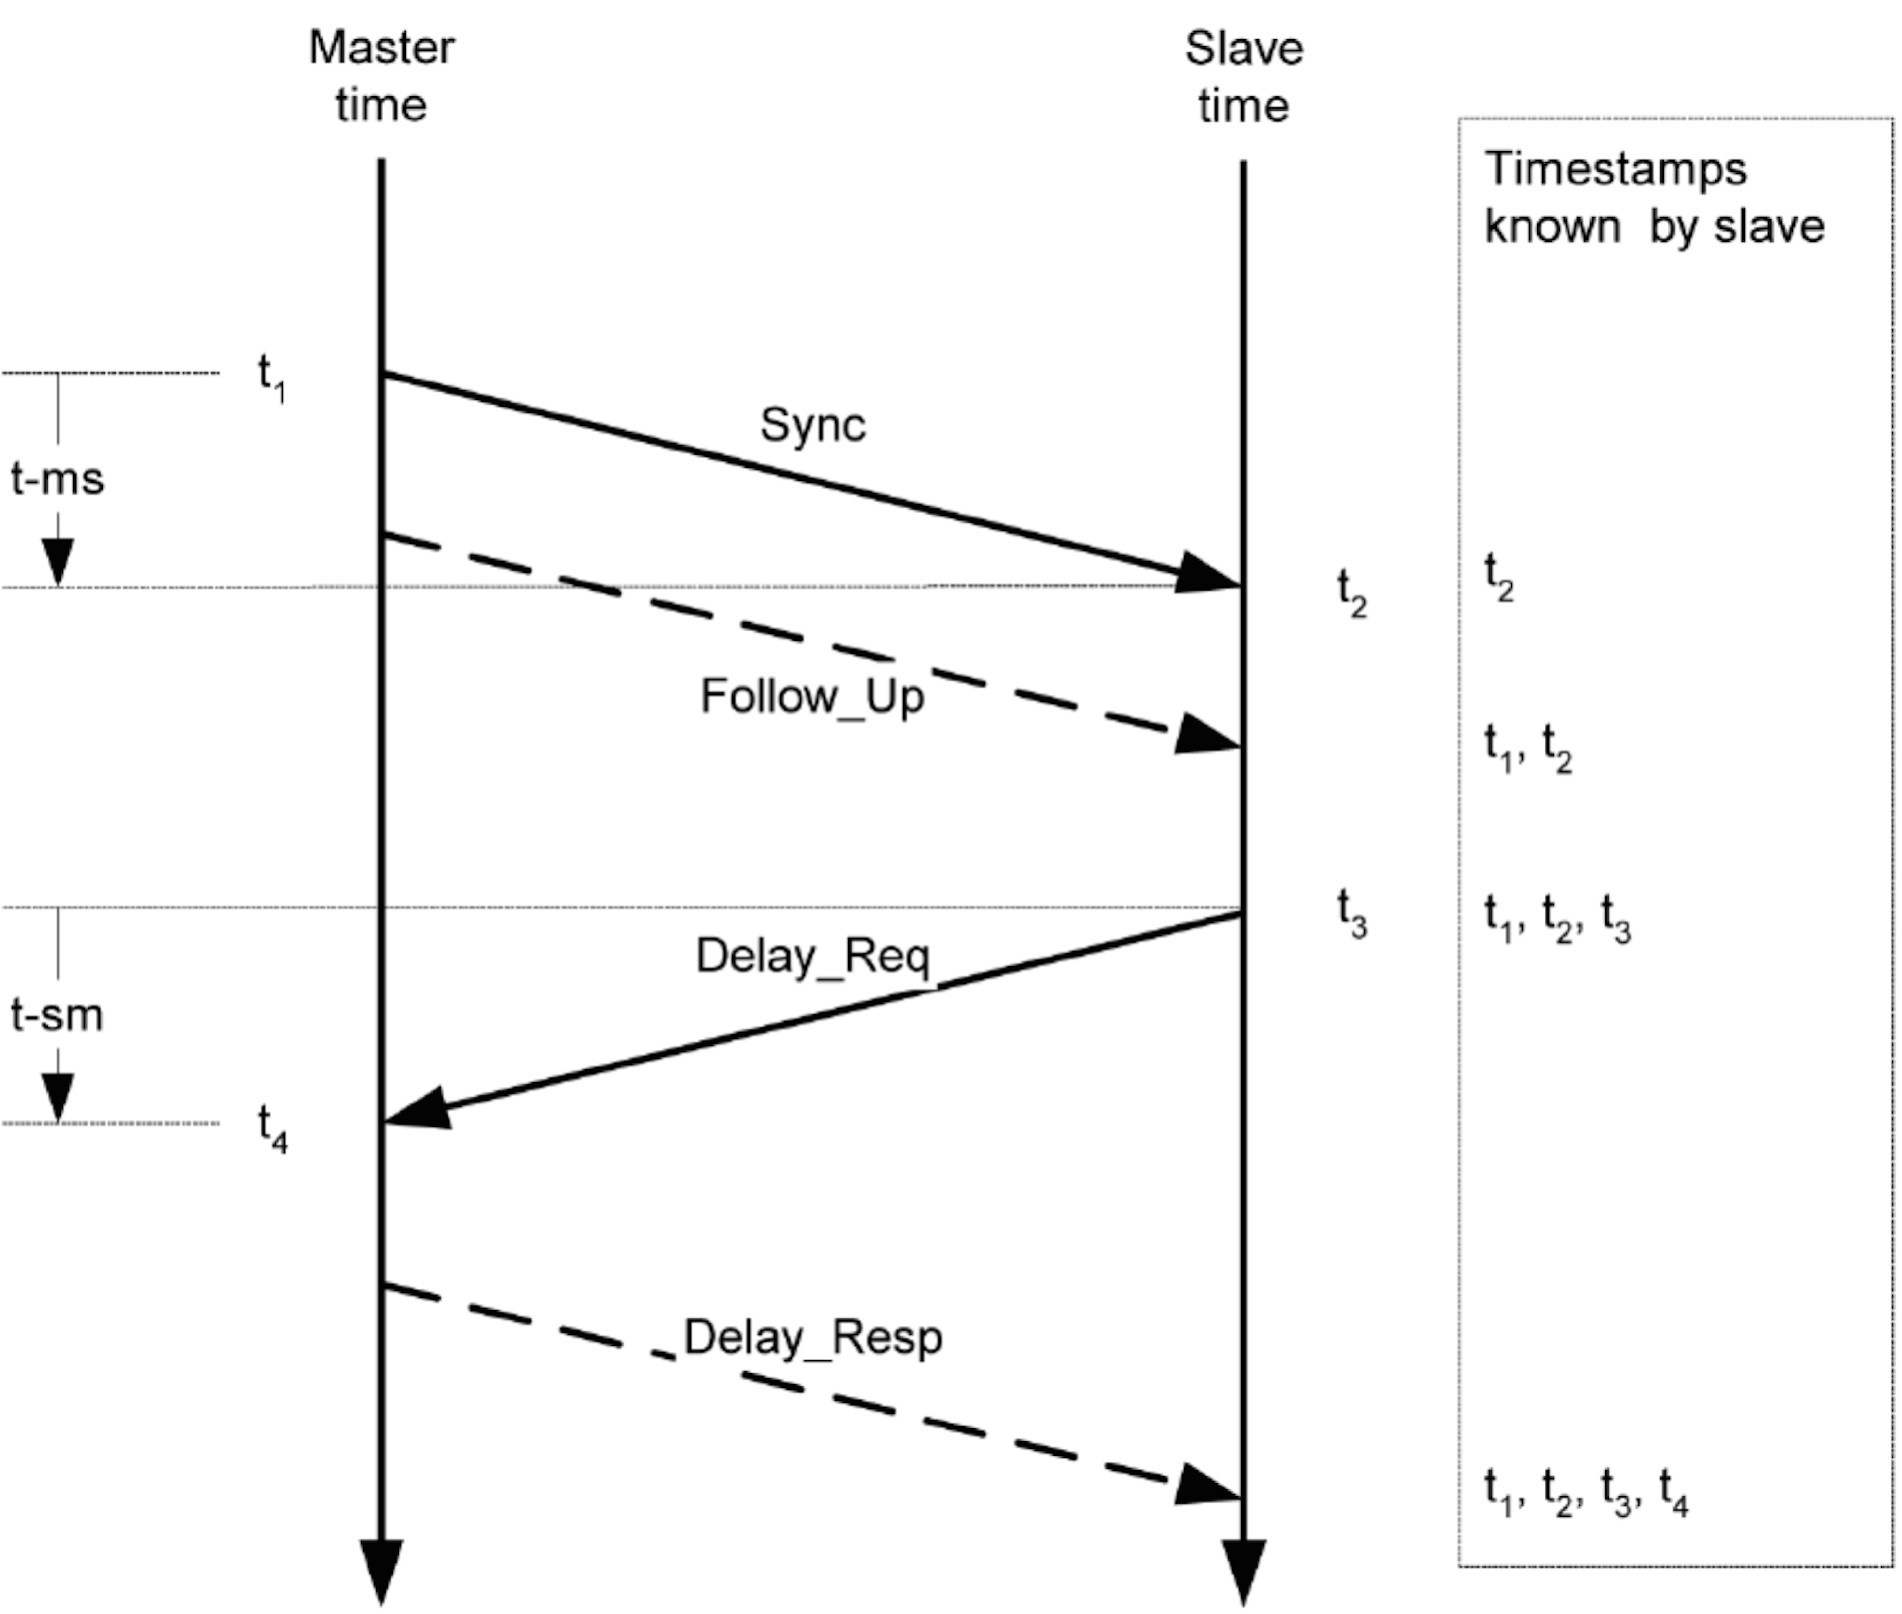
\includegraphics[width=10cm]{process_of_time_sync}
    \bicaption[fig:process_of_time_sync]{时钟同步算法流程图}{时钟同步算法流程图}{Fig}{Method of Time Sync}
  \end{minipage}     
\end{figure}

首先,主时钟会周期性对外发送Sync报文,当该报文离开主时钟时会记录时间戳为t1,若采用硬件时间戳标记的方式则直接把该时间戳存入Sync报文,则无需后续的Follow\_up报文了。

然后,当从时钟接收到Sync报文时,会将接收时间标记为t2。此时,从时钟即获得了Sync报文的发送与接收时间戳t1和t2。那么假设主从时间偏差为$T_{offset}$,主从时钟间网络传输时间为$T_{delay}$,则可以得到下面式子:
\begin{align}
	T_{offset} + T_{delay_1} = t2 - t1
\end{align}

另外,从时钟还会周期性向主时钟发送Delay\_Req报文,假设发送时间为t3,当主时钟收到该报文时,会立即记录下Delay\_Req报文的接收时间t4,并把该接收时间t4存入Delay\_Resp报文中传递回该从时钟。那么此时,从时钟会得到t3和t4两个时间,可得到下面式子:
\begin{align}
	T_{delay_2} - T_{offset} = t4 - t3
\end{align}

此时,根据协议标准中,将往返传输延时视为对称,即:
\begin{align}
	T_{delay_1} = T_{delay_2} = T_{delay}
\end{align}
所以,结合上面几个式子可以得到如下结果:
\begin{align}
	T_{delay} = \frac{(t2 - t1) + (t4 - t3)}{2}
\end{align}
\begin{align}
	T_{offset} = \frac{(t2 - t1) - (t4 - t3)}{2}
\end{align}

通过上面的计算方法,可以得到主从时钟之间的相位偏差$T_{offset}$。然后,还需要计算主从时钟的时钟频率偏差才能实现完整的时钟同步。

为了计算时钟频率偏差,可以采用下面的方法来计算。由于主时钟是隔固定的周期相从时钟发送Sync报文的,所以,对主时钟而言,第i个Sync报文和第(i+1)个Sync报文之间的发送间隔为:
\begin{align}
	\Delta _{master} = T_{m}(k + 1) + T_{delay}(k + 1) - (T_{m}k - T_{delay}k)
\end{align}
对于从时钟而言,两个Sync报文的时间间隔为:
\begin{align}
	\Delta _{slave} = T_{s}(k + 1) - T_{s}k
\end{align}

所以,可以利用上述的比例关系来得到主从时钟的频率偏差。
\begin{align}
	\Delta F = \frac{\Delta _{master}}{\Delta _{slave}}
\end{align}
只需要调节从时钟本地频率扩大$\Delta F$倍就可以实现主从时钟频率一致。

\section{IEEE1588协议实现及分析}
上文中介绍了IEEE1588协议的理论部分,包括主从秩序建立和时钟同步过程。下文会简明扼要地介绍IEEE1588的具体实现过程及相关因素。

\subsection{PTP设备类型}
IEEE1588系统是由PTP设备和非PTP设备结合而成的分布式网络化系统。其中,PTP设备包括普通时钟(Ordinary Clock, OC)、边界时钟(Boundary Clock, BC)、端到端/点到点透明时钟(End-to-End/Peer-to-Peer Transparent Clock, TC)和管理节点。非PTP设备包括普通交换机、路由器及其他底层设备等。

下面对PTP设备作简要介绍:
\begin{itemize}[noitemsep,topsep=0pt,parsep=0pt,partopsep=0pt]
	\item 普通时钟(Ordinary Clock, OC):普通时钟只有一个物理PTP端口,内部包含两个逻辑接口:事件接口主要用来收发含有时间戳的事件报文;通用接口主要用来收发不含时间戳的通用报文。普通时钟指网络中的一般节点,比如电信网基站,或者工业中的测量仪器。
	\item 边界时钟(Boundary Clock, BC):边界时钟包含一个或多个PTP端口,在物理上将一个同步网络划分为多个子网。其每一个端口相当于一个普通时钟,能够引出一条PTP路径,若该端口连接主时钟,则表现从时钟属性;若连接从时钟,则该端口表现主时钟属性。另外,非PTP报文可以通过它来转发,但PTP报文不可以跨越边界时钟。在实际应用中,边界时钟一般安装在路由器、交换机等具有数据收发功能的网络设备上。
	\item 透明时钟(Transparent Clock, TC):透明时钟可以记录报文的进入时间戳和离开时间戳,利用两个时间戳相减得到的相对时间作为驻留时间传递给从时钟,从时钟可以减去该时间从而仿佛报文从未经过该透明时钟,使得波动因素更小。
	\item 管理节点(Management Node):管理节点不需要实现时钟同步功能,它只需要能够对时钟同步进行管理。
\end{itemize}

\subsection{PTP报文介绍}
\subsubsection{PTP报文类型}
PTP协议中的报文分两类,事件(Event)报文和一般(General)报文。下面简单介绍本文使用最多的几种报文。
\begin{itemize}[noitemsep,topsep=0pt,parsep=0pt,partopsep=0pt]
	\item Announce报文:该报文主要用于最佳主时钟算法,报文内部包含描述主时钟所需的数据集,当时钟接收到该报文时,即会调用最佳主时钟算法,比较自身与外部时钟的品质,并根据结果来决定端口的主从状态\supercite{52}。
	\item Sync报文:主时钟周期性对外发送Sync报文,该报文包含了主时钟发送时的时间戳。当从时钟接收到该报文,就会通过offset计算方法来计算出主从时间偏差,并以此来校正自身从而实现同步\supercite{52}。
	\item Delay\_Req和Delay\_Res报文:为了获得主从时钟间的路径传输延时,从时钟会周期性对主时钟发送Delay\_Req报文,当主时钟接收到该报文时,会立即保存接收时间戳,并通过回传Delay\_Res报文把接收时间戳返回给从时钟,用于从时钟的delay值更新\supercite{52}。
\end{itemize}
上面几种报文是本文使用最多的,因此进行了着重介绍。除了上述报文,还有Follow\_Up、PDelay\_Req、PDelay\_Res等报文也非常重要,在此不作过多赘述。

\subsubsection{PTP报文头部格式}
下面分报文头部和报文主体格式进行简单介绍。
所有PTP报文头格式一致,如下图\ref{fig:ptp_message_header}。
其中,各字段含义如下:
\begin{itemize}[noitemsep,topsep=0pt,parsep=0pt,partopsep=0pt]
	\item transportSpecific:标记下一层协议类型,用来区分UDP/IPv6、UDP/IPv4和IEEE802.3;
	\item messageType:标记当前PTP报文类型,包括Sync、Delay\_Req、Follow\_Up、Delay\_Req等;
	\item versionPTP:标记当前PTP版本;
	\item messageLength:标记PTP报文总长度,包含报文头部、报文主体及报文扩展字段;
	\item domainNumber:标记PTP发送端口所属域编号;
	\item flagField:标记单步或双步模式;
	\item correctionField:标记时间修正域,即报文转发时的驻留时间或链路传输延时,该字段为64位有符号整型,意味着它可以使得时间同步精度达到1ns;
	\item sourcePortIdentity:标记发送报文的源端口号,由设备ID及端口ID组成。
\end{itemize}

\begin{figure}[!hbp]
  \centering
  \begin{minipage}[b]{0.6\textwidth}
    \captionstyle{\centering}
    \centering
    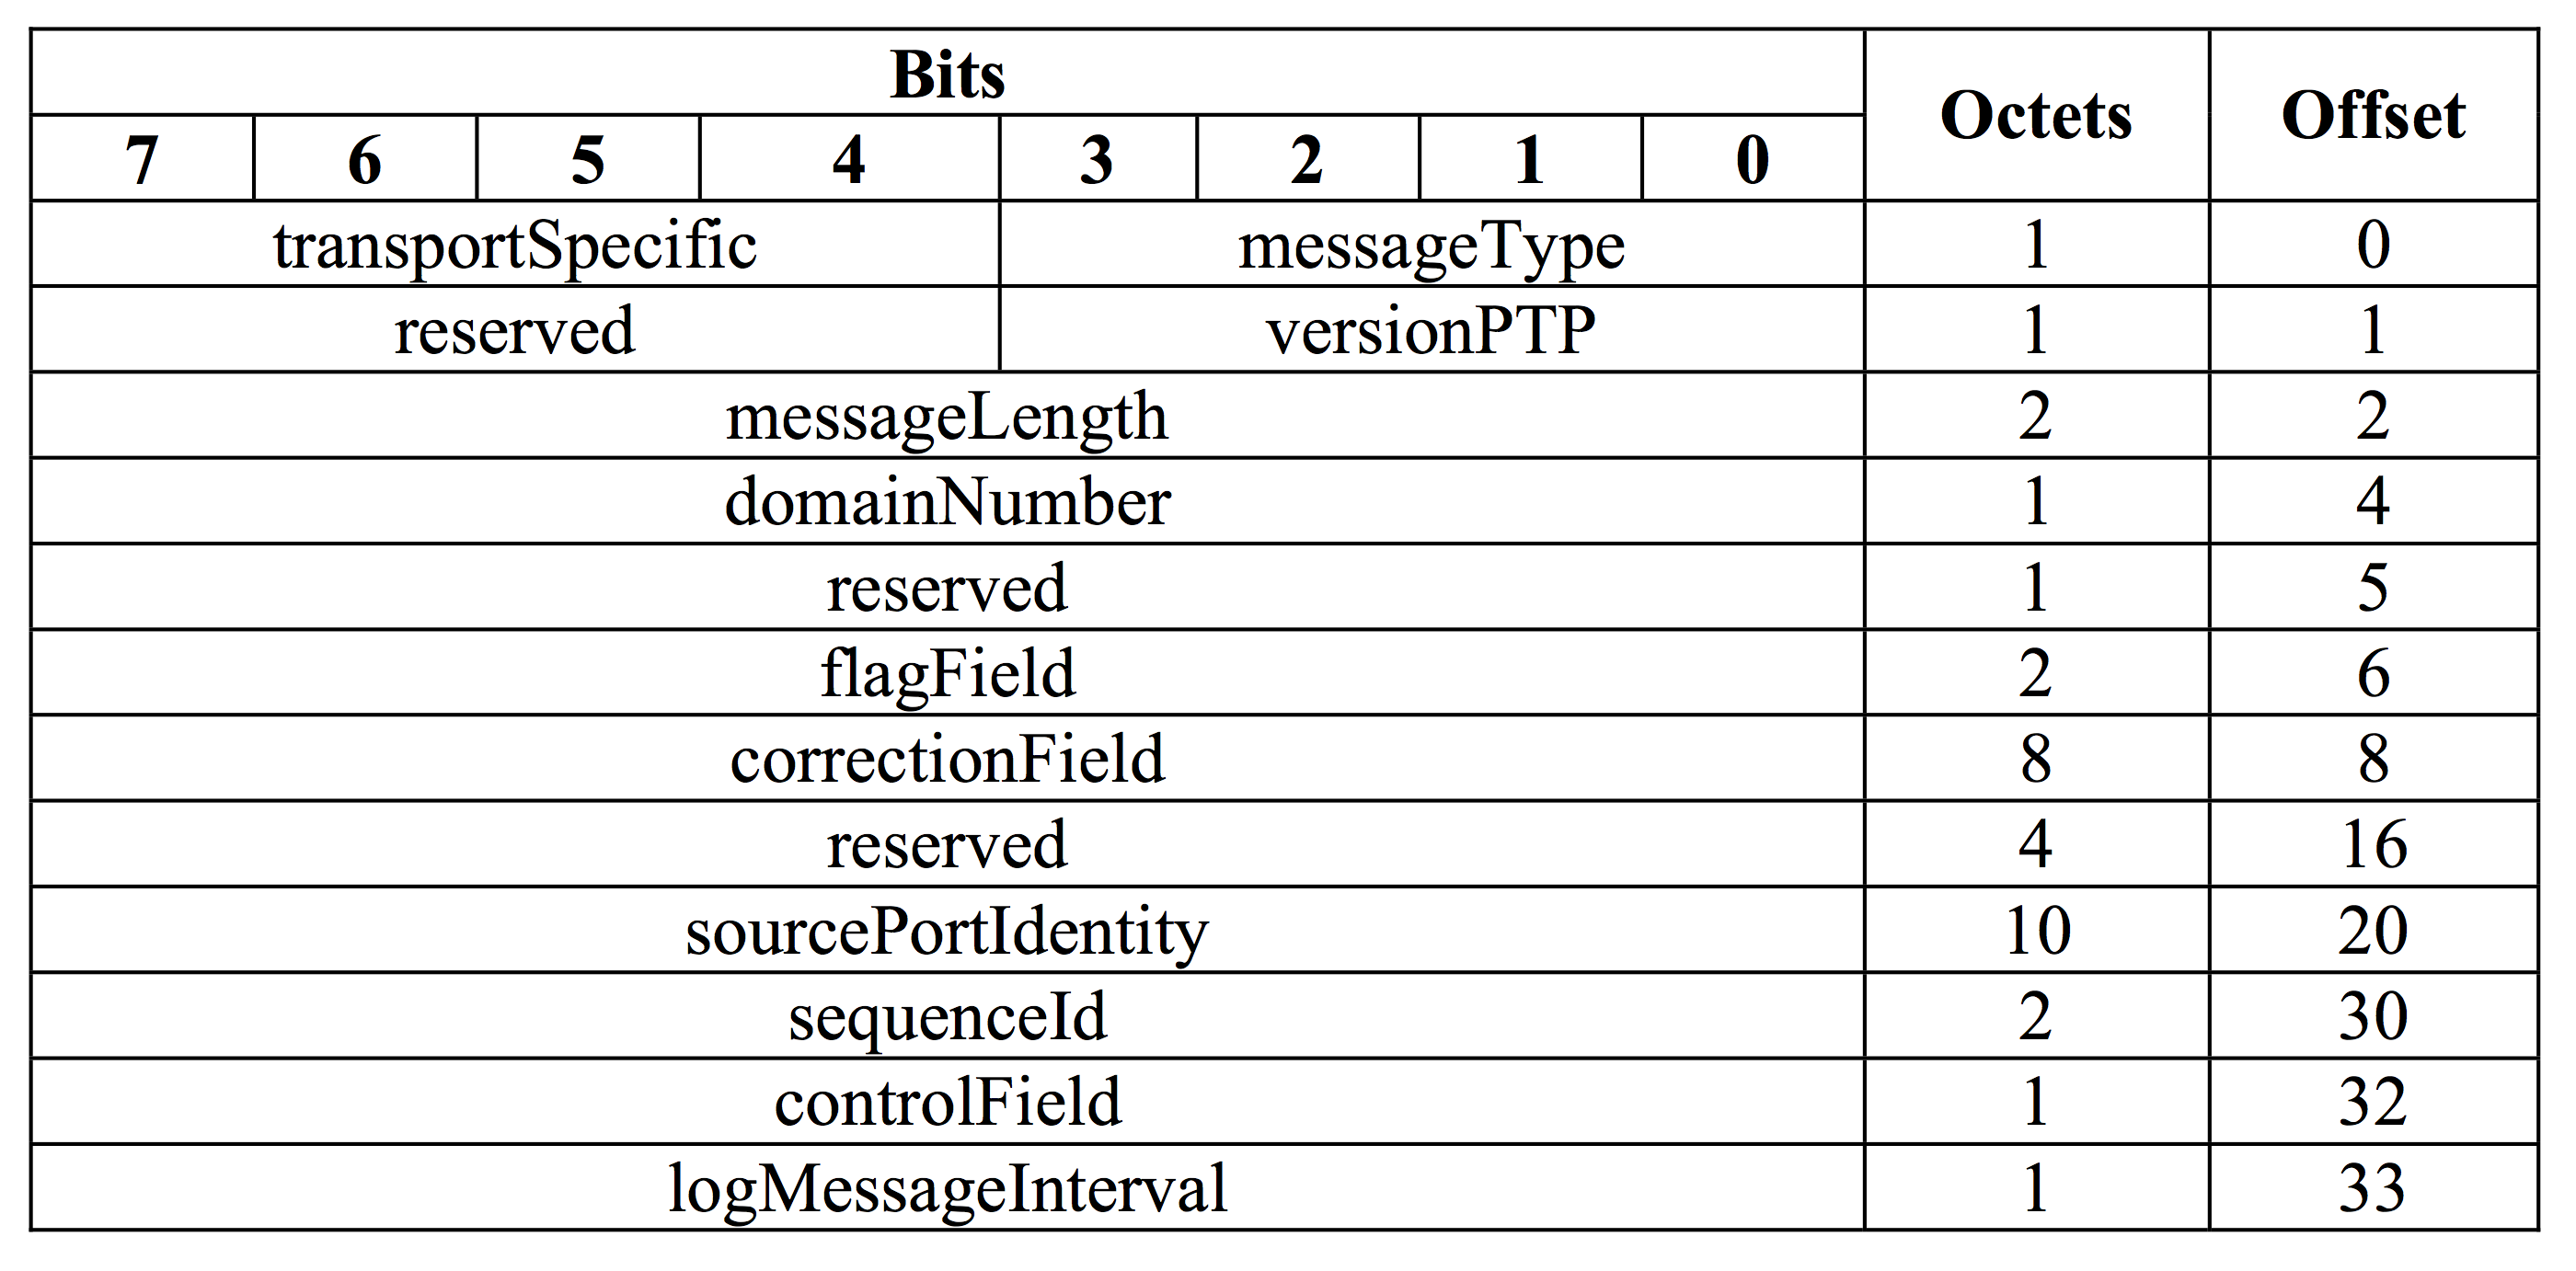
\includegraphics[width=10cm]{ptp_message_header}
    \bicaption[fig:ptp_message_header]{PTP报文头部格式}{PTP报文头部格式}{Fig}{The Style of PTP message Header}
  \end{minipage}     
\end{figure}

\subsubsection{PTP报文主体格式}
PTP报文中的Sync和Req\_Delay两种报文主体主要包括了时间戳信息:NanosecondsField和SecondsField,分别表示时间戳的秒部分和纳秒部分。
\begin{figure}[!hbp]
  \centering
  \begin{minipage}[b]{0.6\textwidth}
    \captionstyle{\centering}
    \centering
    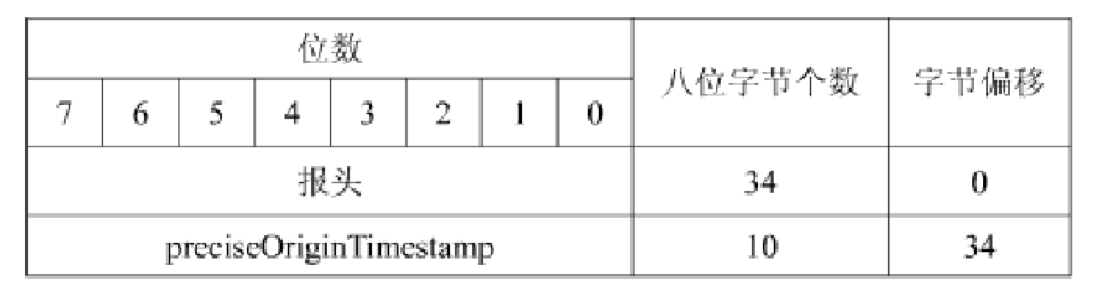
\includegraphics[width=10cm]{ptp_message_content}
    \bicaption[fig:longcaptiongood]{PTP报文主体格式}{PTP报文主体格式}{Fig}{The Structure of Sync Req\_Delay message content}
  \end{minipage}     
\end{figure}

另外,对于Announce报文,其主体内容如图\ref{fig:ptp_announce_message_content}所示:

\begin{figure}[!hbp]
  \centering
  \begin{minipage}[b]{0.6\textwidth}
    \captionstyle{\centering}
    \centering
    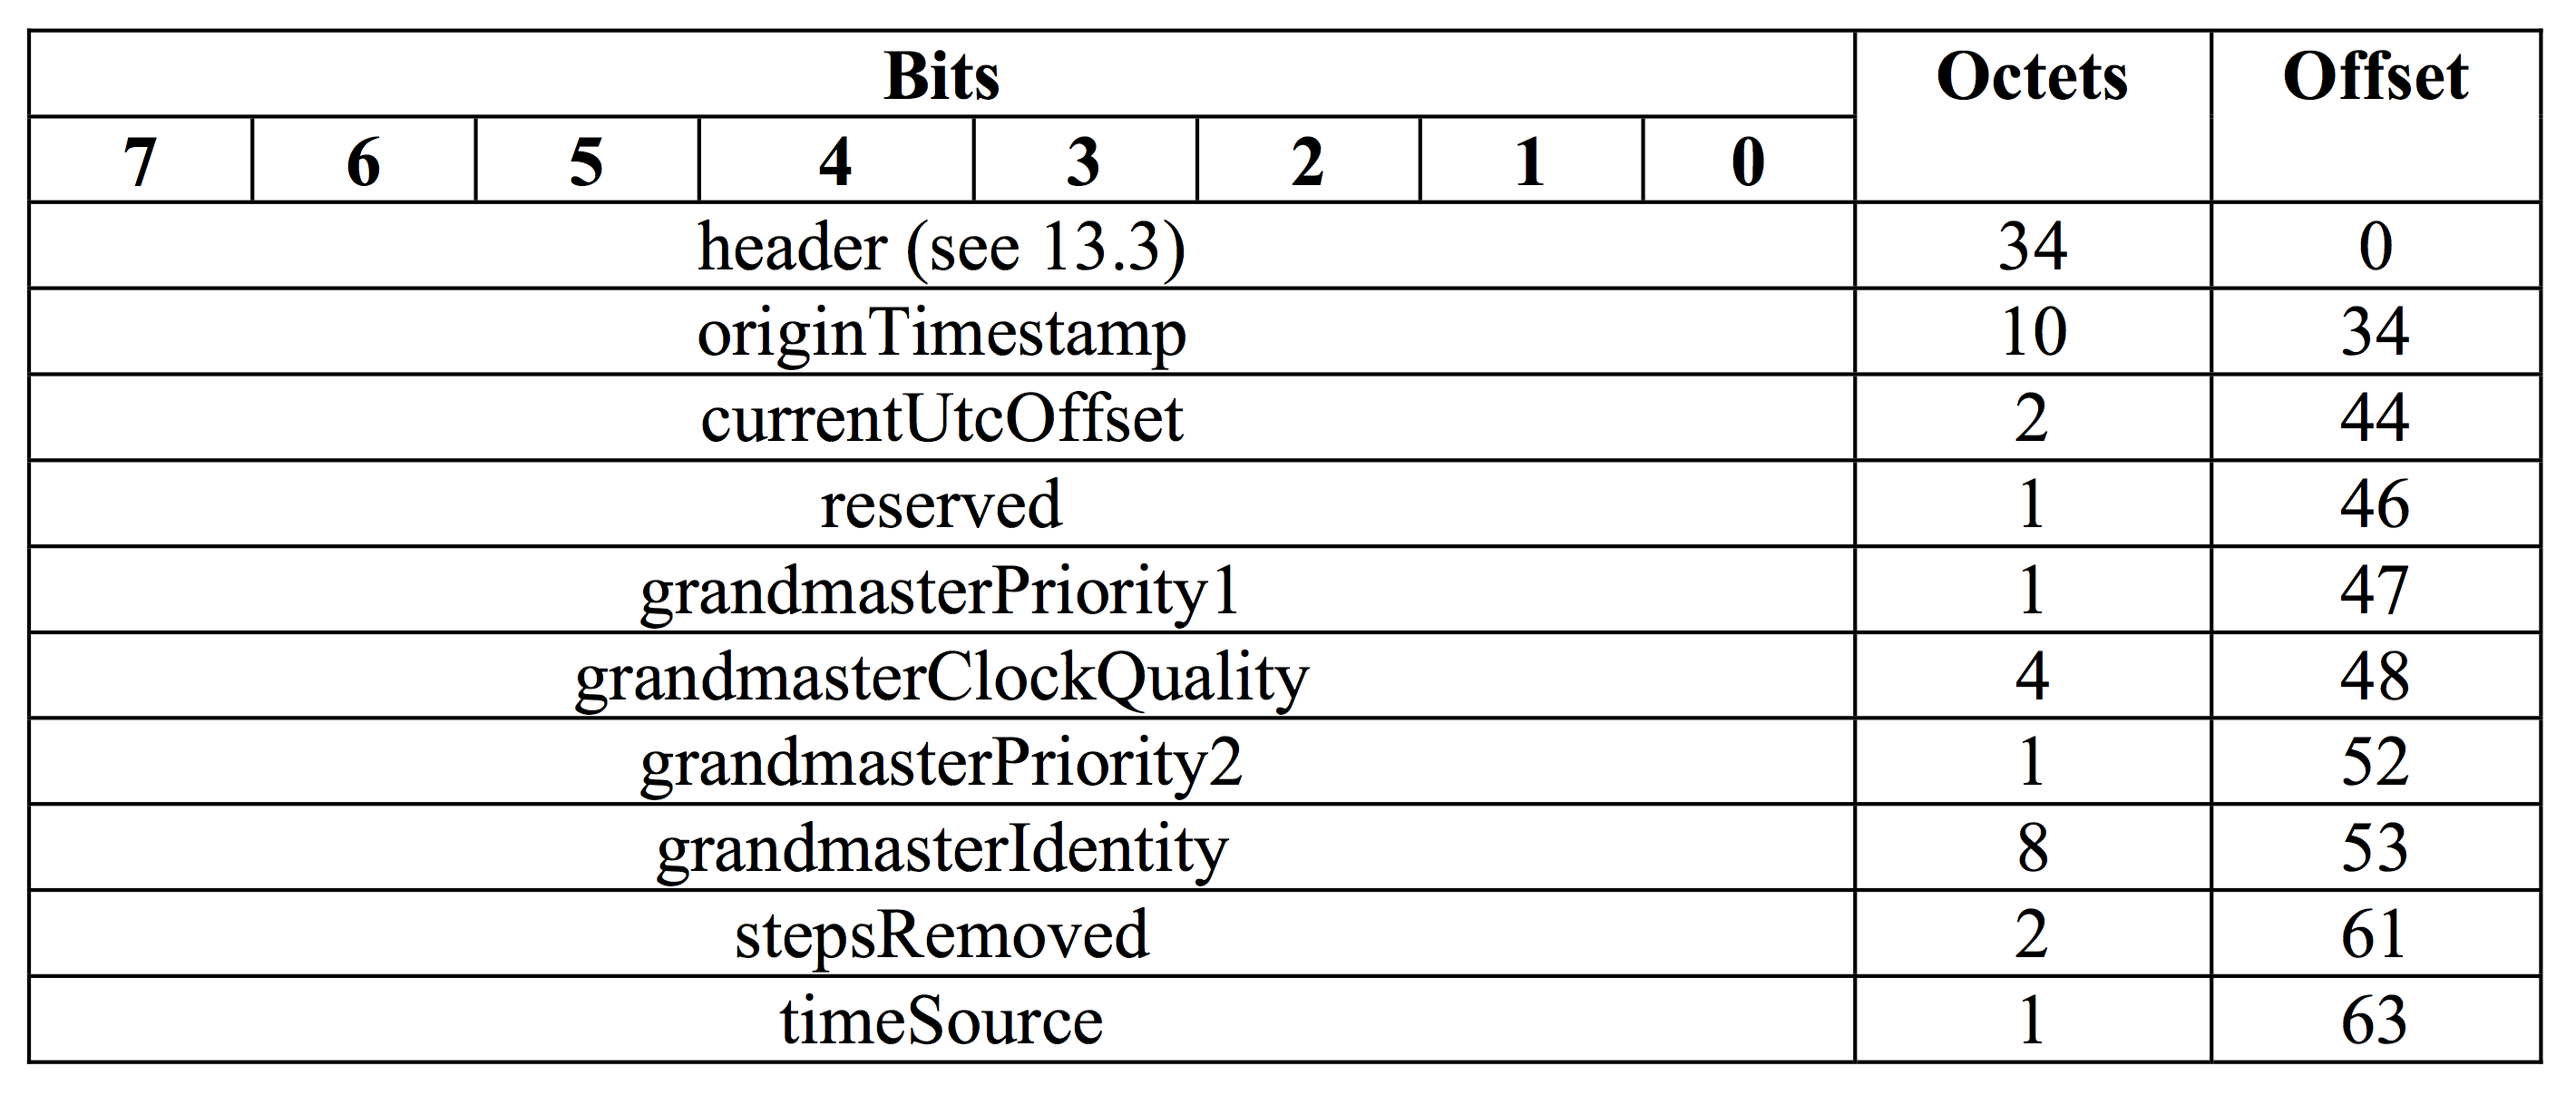
\includegraphics[width=10cm]{ptp_announce_message_content}
    \bicaption[fig:ptp_announce_message_content]{Announce报文主体格式}{Announce报文主体格式}{Fig}{The Structure of Announce message content}
  \end{minipage}     
\end{figure}

其中,grandmasterPriority1、grandmasterClockQuality、grandmasterPriority2和grandmasterIdentity等数据都是用来表示Grand Master的时钟质量,对外发送以让其他时钟能够进行数据集比较算法,然后依靠端口状态变化规则来建立整个系统的主从状态。

\section{PTP报文封装与传输周期对同步精度的影响分析}

\subsection{PTP报文封装传输过程及其对同步精度的影响分析}
首先,一般来讲会在应用层准备PTP协议报文,把当前时间戳信息作为传递数据打包进去并传递给传输层;然后,操作系统按照网络协议栈将应用层数据依次打包进入UDP传输层报文和IP网络层报文;然后从网络层发送给数据链路层,该层会为报文添加以太网帧的首部和尾部形成完整的以太网报文,发送给物理层硬件发送出去\supercite{54}。

\subsection{PTP报文传输周期及其对同步过程的影响分析}
在同步过程中,最重要的便是offset值和delay值的计算,这直接涉及到同步结果的准确性和稳定性;另外还有最初主从秩序建立的快速性也非常重要。所以,下面简单介绍相关的时间周期和超时事件,并分析其对同步过程的影响。
\begin{itemize}[noitemsep,topsep=0pt,parsep=0pt,partopsep=0pt]
	\item Announce报文周期:在实际应用中,该周期值保存在portDS.logAnnounceInterval里,所表示的实际周期为$2^{portDS.logAnnounceInterval}$。协议中规定Announce报文默认发送间隔为2s,可配置范围为1s-16s,采用多播方式。当从时钟接收到该报文,若端口为Slave状态,则会更新本地数据集。
	\item Sync报文周期:该报文周期值保存在portDS.logSyncInterval中,取值范围为-1-1,对应的实际周期为0.5s-2s。每个Master端口都会持续周期性发送该报文,而每次slave端口收到Sync报文就会触发在本地的同步计算并执行校正。对于该值的选取也应该慎重考虑,如果该周期过大,则会使的从时钟偏离太大而失去同步效果;若该周期太小,则会严重加剧网络流量负载,从时钟处于不断的调整波动之中。
	\item Delay\_Req报文周期:该报文周期值保存在portDS.logMinDelayReqInterval中,取值范围为0-5,对应的实际周期为1s-32s,默认值为1s。该报文主要用来更新链路延时delay值。对于该值的选取也应该慎重考虑,如果周期过小,则会给主时钟增加过多的负载压力,加剧网络流量负载;若周期过大,则有可能导致上一次的delay与当前实际delay值出现严重偏差,从而导致offset值偏差较大,严重破坏同步精度。理想的周期应该在区间[0, $2^{portDS.logMinDelayReqInterval+1}$]中均匀分布。
\end{itemize}

\section{IEEE1588实际应用中存在的问题及研究目标}
在上文中,主要介绍了IEEE1588协议的实现原理。根据对原理如时钟同步算法的分析研究,再加上PTP协议在工业实际中的精度表现,可以发现该协议中仍然存在一些影响精度的因素,而且,如果希望实际精度能够达到微秒级甚至纳秒级,就不得不对这些因素进行深入的研究。下面将结合IEEE1588的实现原理及实际表现,提出其中存在的固有弊病和漏洞,正是这些问题导致了实际运行中的同步精度难以达到亚微秒级。

\subsection{链路延时不对称}
\label{sec:1588_problem_1}
在IEEE1588协议中,当计算主从时钟偏差offset时,需要先获取链路传输延时delay。在协议中该延时的计算方法是直接假设前后两次传输延时相等,从而通过取平均计算出offset。然而实际上,前后两次的传输路径往往并不对称,经过分析,可以发现以下几个导致往返的链路传输延时不一致的因素\supercite{55}。
\begin{itemize}[noitemsep,topsep=0pt,parsep=0pt,partopsep=0pt]
	\item 排队堵塞:当报文在传输中经过中间交换机或路由器时,由于网络负载的不可预知性,无法知道报文在中间交换机上的排队时间,当网络流量良好时,报文可以直接传递过去;而当网络负载较大,可能导致很长的报文排队时间。另外,即使报文可以不用排队,由于协议栈的存在,报文仍然需要经过解包和打包的过程,而这两个过程的消耗时间都与操作系统的调度和协议栈处理过程有关。因此,报文传递过程中穿越交换机时排队和堵塞时间的随机性会导致延时不对称\supercite{46}。
	\item 传输抖动:在网络系统中,所有信息的传递过程所消耗的时间会存在固有的抖动,这时无法避免的。
	\item 网络拓扑结构变化:当拓扑结构突然发生变化,报文传输的路径也就不同了,这必然导致往返链路时延完全不同。
	\item delay与当前真实延时不匹配:因为delay的计算依靠Delay\_Req报文周期,而offset的计算又是依靠Sync报文周期,两者一般并不匹配。所以会导致在计算offset所使用的delay是过去的值,与当前真实的delay值可能并不一致。
\end{itemize}

上述几种现象的存在,都会导致往返的两次延时不一致,所以说,在高同步精度的要求下,真实的传输延时绝对不能简单的假设相等。

对于网络延时的研究,也正是本文的重点内容。在接下来的内容中,文章会对上述所提到的几种因素进行拆解分析,同时,从数学统计的角度,把所有历史延时数据作为样本,采用多个统计方法来对数据进行处理和消除干扰,从而得到稳定的同步数据。

\subsection{主从时钟源频率漂移}
由于主时钟在发送Sync报文时的偏差值Offset\_1与从时钟最后接收Delay\_Respo报文时的偏差值Offset\_2是不完全一致的,所以最终计算出来的offset并不完全等于真实的Offset\_2。所以这会导致同步精度变差。因此下面将利用上面的Sync报文统计样本,采用统计方法来计算主从时钟源频率偏差,从而对从时钟进行校正。

\subsection{时间戳的精确度}
\label{sec:1588_problem_2}
在上文中的报文的封装传输过程已经提到,由于在协议栈中传递所带来的延时,导致物理层之上的时间戳往往不能真实反映报文的发送时间或接收时间,若直接使用这种时间戳来进行计算,那么从根本上就带来了误差\supercite{53}。所以,如果一些设备采用的是软件时间戳方式,那么报文的封装和解包过程就势必会对真实的时间戳产生偏差,这种时间戳精确度上所带来的误差是不可忽视的。

不过,在实际参与的交换机项目中,采用的是支持硬件时间戳的设备,该设备能够直接在数据链路层与物理层之间为报文添加时间戳,从而保证了时间戳的精确度,因此,在本文中,并不会对该因素作过多深入的探讨和研究。

